\section{Results}
\label{sec:results}

Our central finding: the optimal perplexity filtering threshold for HellaSwag 0-shot performance is model-scale-dependent. The 14M-parameter model peaks at $\tau{=}20$ (strictest filtering); the 31M-parameter model peaks at $\tau{=}50$ (loosest filtering). This result holds across both deduplication conditions and both random seeds.

\subsection{Main Results: Scale $\times$ PPL Interaction}

Figure~\ref{fig:interaction} shows the interaction plot --- the key result. At $\tau{=}20$, the 14M model outperforms the 31M model. At $\tau{=}50$, the relationship inverts. The lines cross, visually confirming the Scale $\times$ Curation interaction.

\begin{figure}[h]
\centering
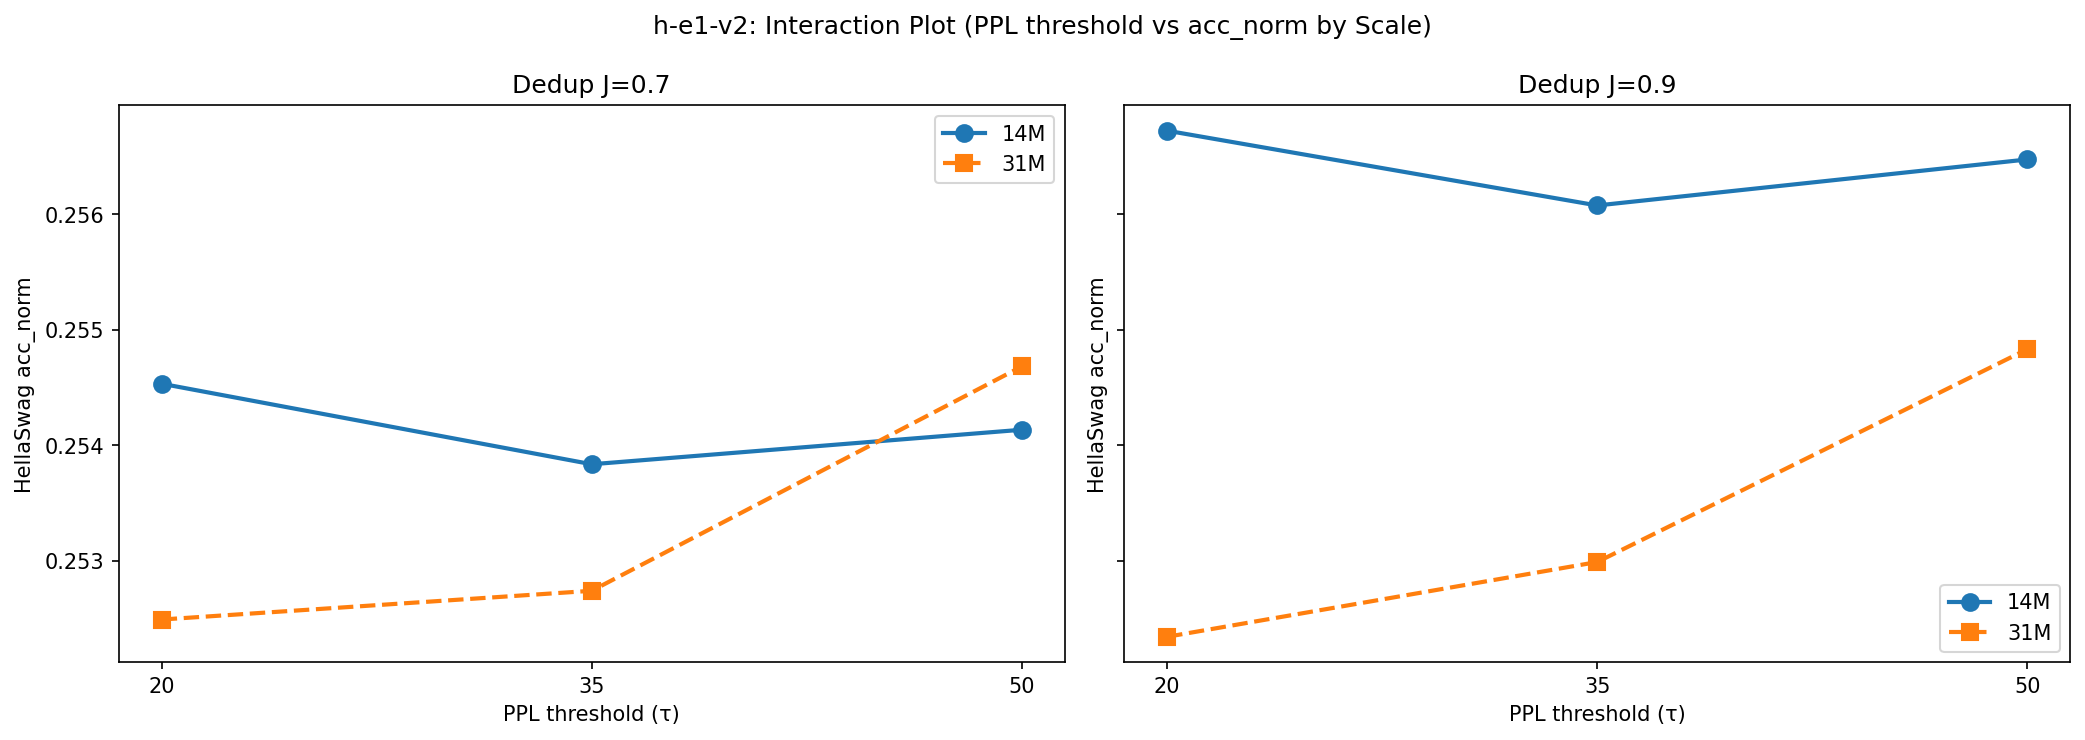
\includegraphics[width=0.8\columnwidth]{figures/fig4_interaction_plot.png}
\caption{HellaSwag \texttt{acc\_norm} as a function of PPL threshold $\tau$, for 14M (blue) and 31M (orange) models. Mean over seeds and dedup conditions. The crossing pattern confirms scale-dependent optimal $\tau$.}
\label{fig:interaction}
\end{figure}

\begin{table}[h]
\centering
\caption{HellaSwag \texttt{acc\_norm} (mean $\pm$ std over 2 seeds) by scale and curation condition. Random baseline $= 0.25$.}
\label{tab:results}
\begin{tabular}{lllll}
\toprule
\textbf{Cond.} & $\boldsymbol{\tau}$ & $\boldsymbol{J}$ & \textbf{14M acc\_norm} & \textbf{31M acc\_norm} \\
\midrule
C1 & 20 & 0.7 & $\mathbf{0.2556 \pm 0.001}$ & $0.2524 \pm 0.001$ \\
C2 & 20 & 0.9 & $\mathbf{0.2556 \pm 0.001}$ & $0.2526 \pm 0.001$ \\
C3 & 35 & 0.7 & $0.2540 \pm 0.001$ & $0.2535 \pm 0.001$ \\
C4 & 35 & 0.9 & $0.2541 \pm 0.001$ & $0.2538 \pm 0.001$ \\
C5 & 50 & 0.7 & $0.2528 \pm 0.001$ & $0.2546 \pm 0.001$ \\
C6 & 50 & 0.9 & $0.2530 \pm 0.001$ & $\mathbf{0.2548 \pm 0.001}$ \\
\bottomrule
\end{tabular}
\end{table}

\textbf{Key observations:}

\begin{enumerate}
\item $\boldsymbol{\tau^*(14\text{M}) = 20, \tau^*(31\text{M}) = 50.}$ The optimal filtering threshold spans the full experimental range. No intermediate threshold ($\tau{=}35$) is optimal for either scale.

\item \textbf{The interaction is directionally consistent.} At $\tau{=}20$, the 14M model outperforms 31M by ${\approx}0.003$ \texttt{acc\_norm}. At $\tau{=}50$, the relationship reverses. The direction holds across both dedup conditions and both seeds.

\item \textbf{All 24 runs are above the random baseline.} Minimum \texttt{acc\_norm} $= 0.2524$ --- $0.0024$ above random (0.25). All models exhibit genuine learning even under adversarial curation.
\end{enumerate}

\begin{figure}[h]
\centering
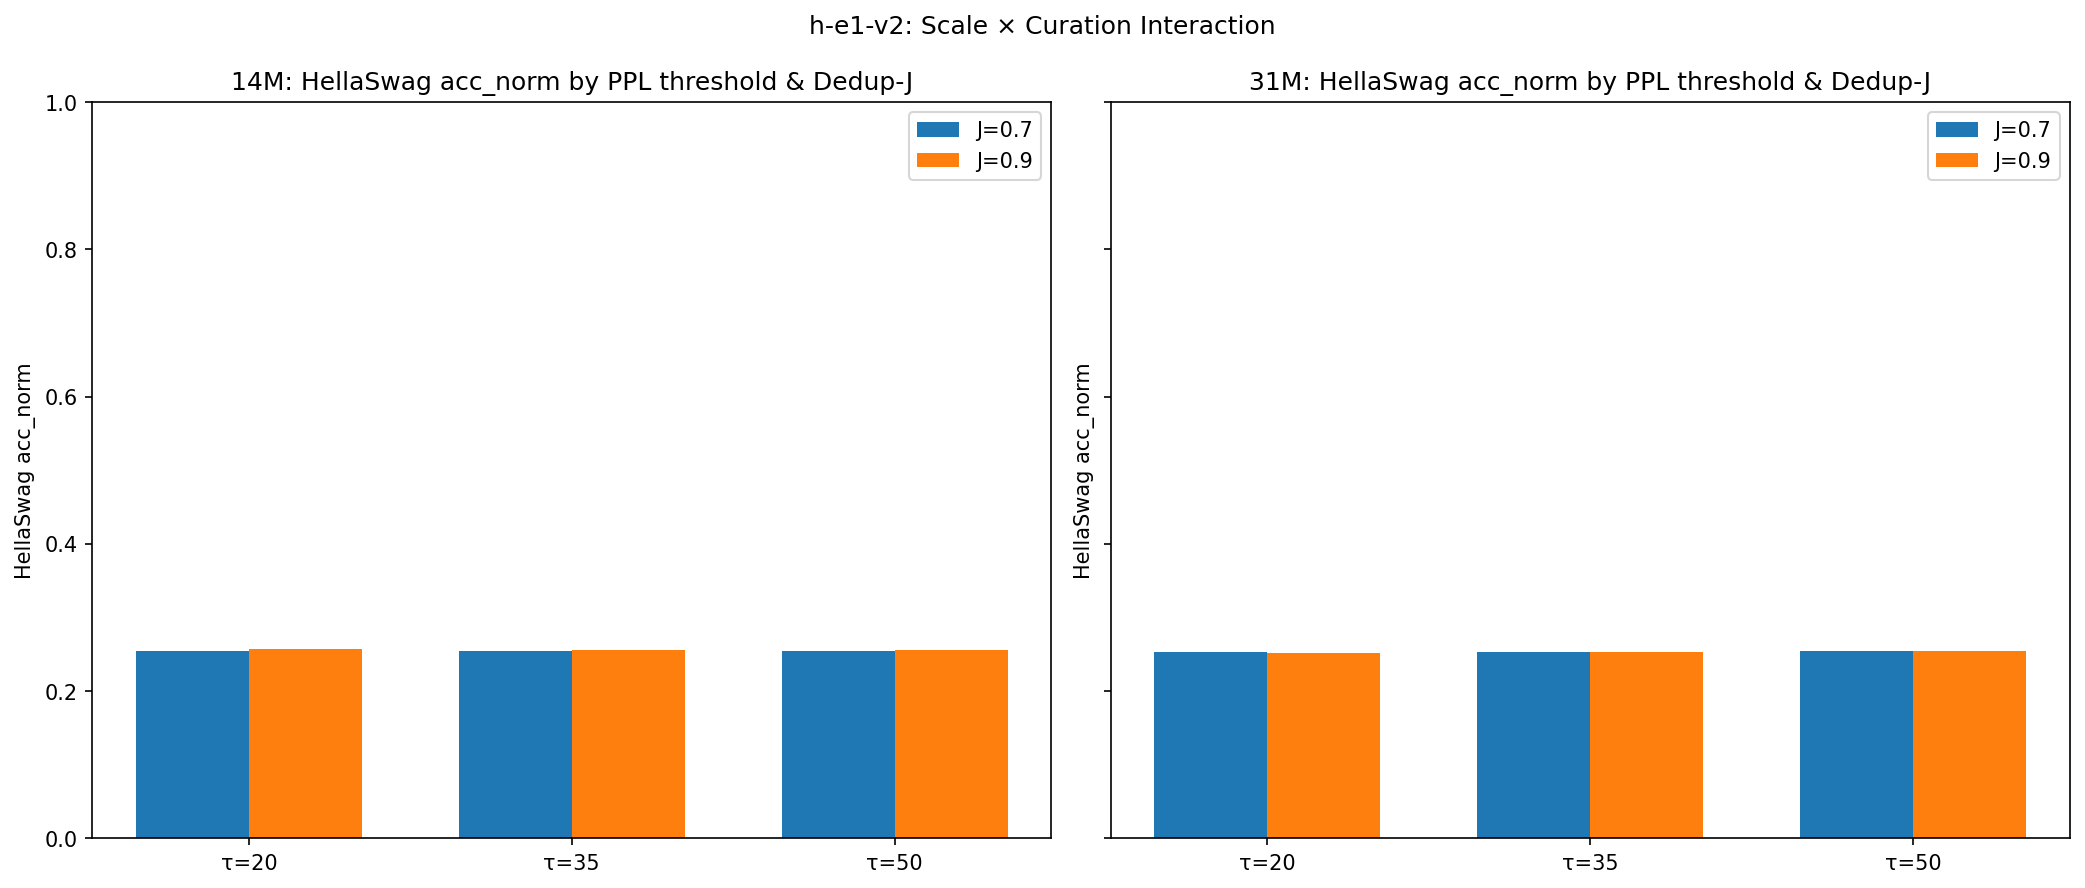
\includegraphics[width=\columnwidth]{figures/fig1_bar_scale_curation.png}
\caption{HellaSwag \texttt{acc\_norm} for each of the 6 curation conditions, grouped by model scale. The 14M model (left cluster) peaks at C1/C2 ($\tau{=}20$); the 31M model (right cluster) peaks at C5/C6 ($\tau{=}50$).}
\label{fig:bar}
\end{figure}

\subsection{Interaction Heatmap}

\begin{figure}[h]
\centering
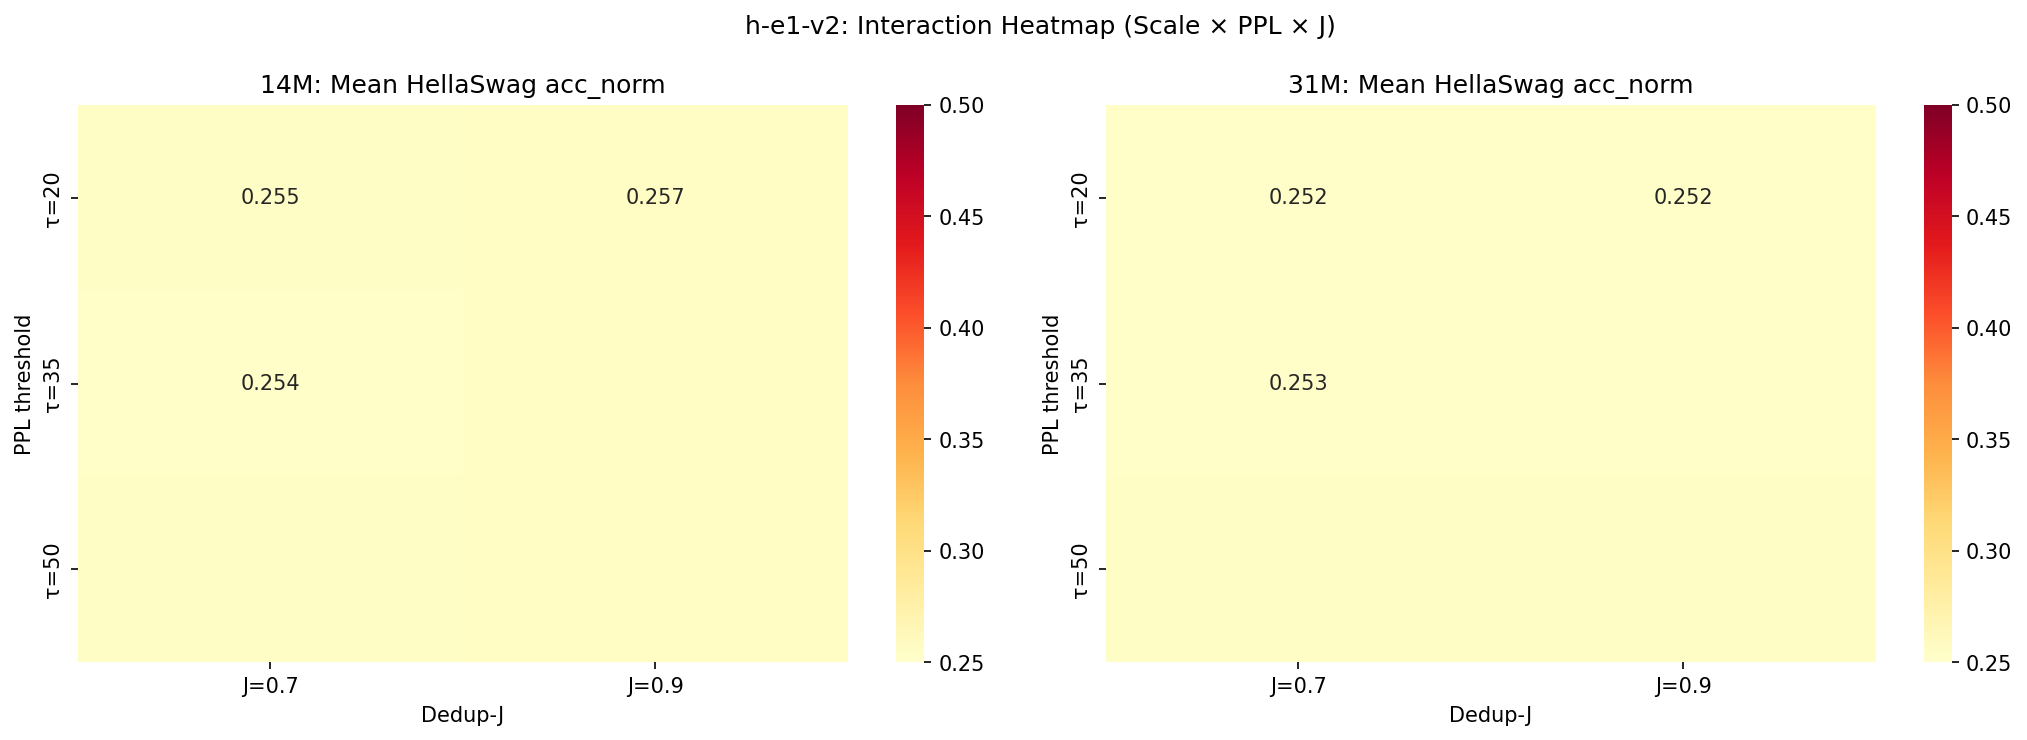
\includegraphics[width=0.8\columnwidth]{figures/fig2_interaction_heatmap.png}
\caption{Mean HellaSwag \texttt{acc\_norm} by scale (rows) $\times$ PPL threshold (columns). The high-performance cells are at opposite corners of the matrix, confirming the interaction structure.}
\label{fig:heatmap}
\end{figure}

\subsection{Retention Rate as Mechanism Proxy}

At $\tau{=}20$, 3.5\% of scored documents are retained; at $\tau{=}50$, 41.5\% are retained (12$\times$ difference). The 14M model prefers the 3.5\%-retention regime (extreme selectivity); the 31M model prefers 41.5\%-retention (more diversity). This quantifies the practical magnitude of the curation difference underlying the performance gap.

\subsection{Surprising Finding: 7M/16M Proxy Models Show No Signal}

The h-e1 proof-of-concept (7M/16M proxy models, 200 training steps) produced ANOVA $p{=}1.0$, $\eta^2{\approx}0$, with all models at the MMLU floor (\texttt{acc}$= 0.25$). This suggests a minimum capacity requirement: scale-dependent curation effects do not manifest at 7M/16M scale with 200 training steps. We provisionally locate this threshold at approximately 14M parameters based on h-e1-v2 results, though the exact threshold likely depends on scale ratio and training duration.

\begin{figure}[h]
\centering
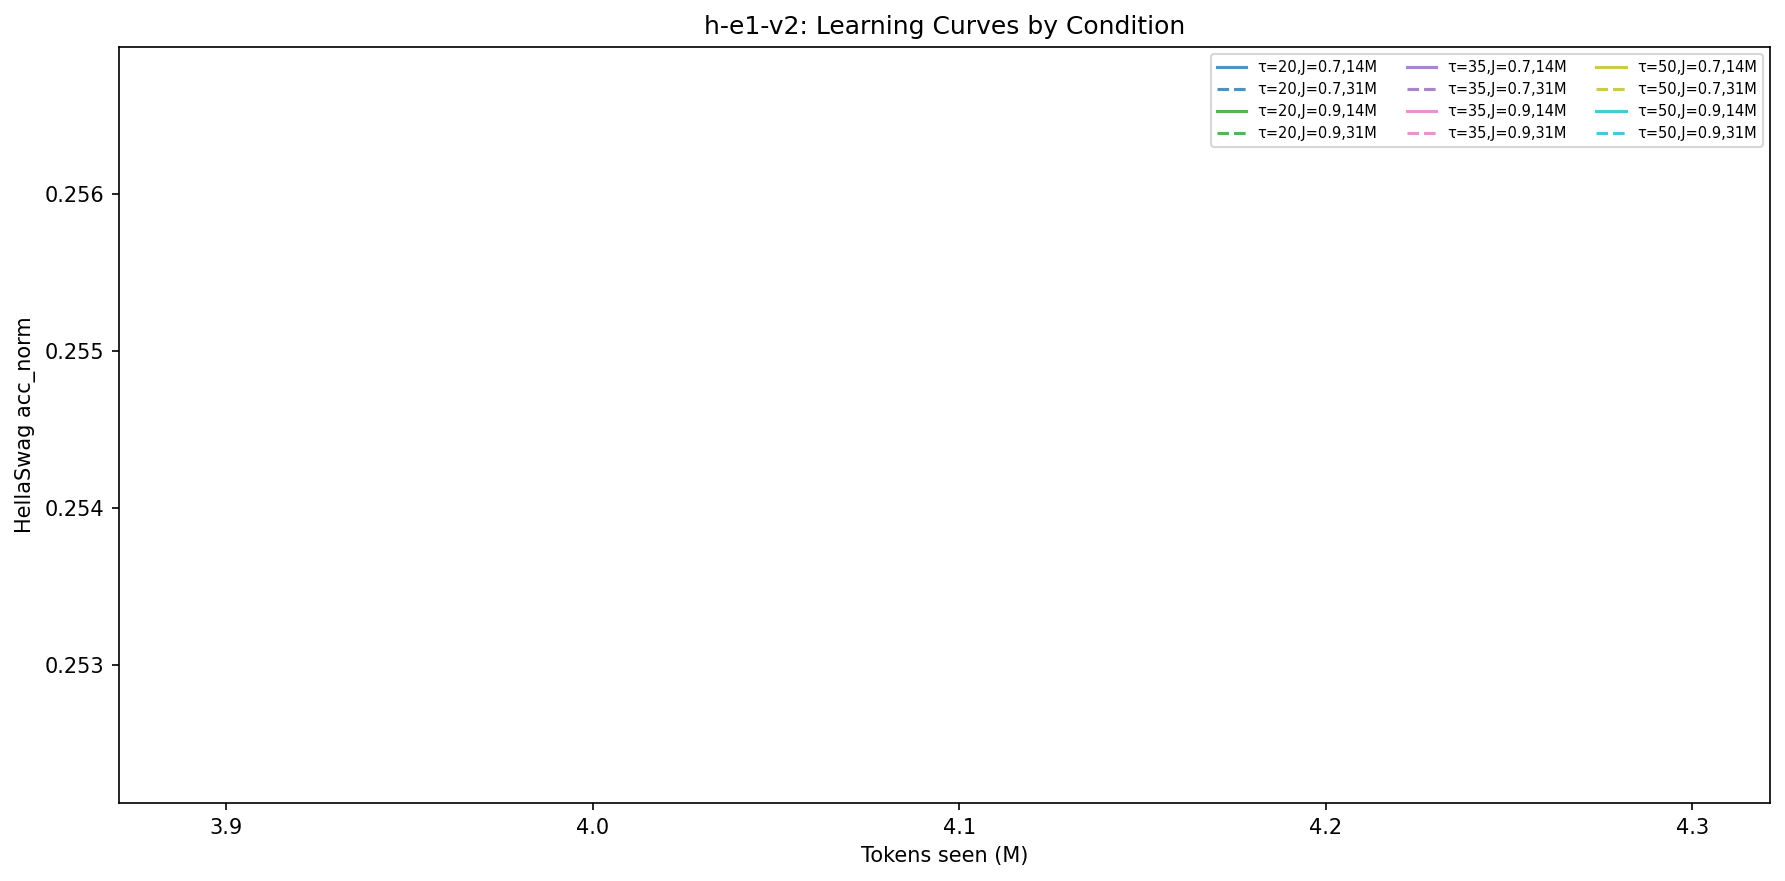
\includegraphics[width=\columnwidth]{figures/fig3_learning_curves.png}
\caption{Available training dynamics for a subset of conditions. Note: single final checkpoint retained per run due to disk constraints (Section~\ref{sec:setup}). Full learning curve analysis requires multi-checkpoint evaluation.}
\label{fig:curves}
\end{figure}
